\section{Planteamiento problema}
El uso de plataformas educativas, buscadores, bibliotecas digitales, procesadores de texto, aplicaciones de
colaboración y asistentes basados en inteligencia artificial se ha diversificado. No obstante, dentro de una
población universitaria pueden existir diferencias en frecuencia, finalidad, percepción de utilidad, habilidades
digitales y dificultades de acceso. Sin datos recogidos de los propios estudiantes, no es posible establecer cuáles
herramientas predominan ni qué barreras son más frecuentes en el grupo concreto que se pretende estudiar.

El problema de investigación consiste en la falta de una caracterización sistemática, para la población
que finalmente se delimite de las herramientas digitales que los estudiantes utilizan con fines académicos, la
frecuencia con que las emplean, sus principales propósitos y las dificultades que reportan. La propuesta no afirma
que exista una magnitud conocida de esta brecha; precisamente plantea medirla mediante un instrumento
estructurado.


\begin{callout}
\textbf{Pregunta de investigación}

¿Qué herramientas digitales utilizan los estudiantes
universitarios de Bogotá, con qué frecuencia y para
qué actividades académicas?
\end{callout}


\begin{figure}[H]
    \caption{Uso de herramientas digitales en estudiantes universitarios de Bogotá, Colombia}
    \label{fig:conectividad-hogares}

    \centering
    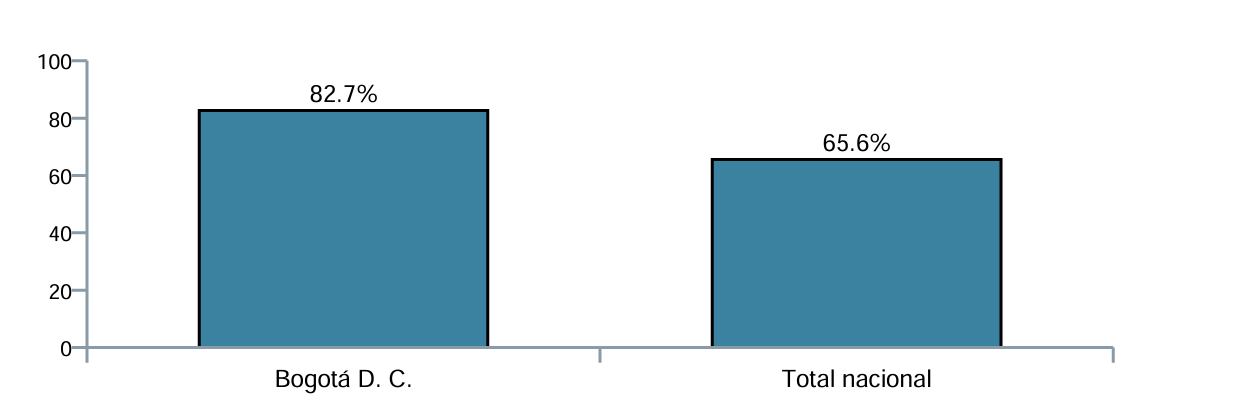
\includegraphics[width=1\textwidth]{assets/images/grafico-conect-Internet.png}

    \par\smallskip
    \begin{minipage}{0.8\textwidth}
        \footnotesize
        \textit{Nota.} Porcentaje de hogares con conexión a internet en 2024. La cifra no corresponde a estudiantes ni mide uso académico. Fuente: DANE \parencite{dane2025entic}, boletín técnico de la ENTIC Hogares 2024.
    \end{minipage}
\end{figure}
\subsection{Justificación del problema}
Una caracterización puede ayudar a reconocer qué herramientas forman parte de las prácticas de estudio,
cuáles se utilizan de manera ocasional y qué dificultades reportan los participantes. Esta información podría servir
como línea base para futuras acciones institucionales; no permitiría, por sí sola, concluir que una herramienta
causa mejores calificaciones o mayor aprendizaje.